\documentclass[12pt]{book}
\usepackage[dvipsnames]{xcolor}
\usepackage{amssymb,latexsym}
\usepackage{graphicx}

%\usepackage[spanish,mexico,es-nolayout]{babel}
\usepackage[utf8]{inputenc}
\usepackage{amsmath}
%\usepackage{amssymb}
\usepackage{amsthm}
%\usepackage{graphicx}
\usepackage{color}
\usepackage{tikz}
\usepackage{tkz-berge}
\usepackage{makeidx}
\usepackage{url}
\usepackage{xspace}
\usepackage{tocbibind}
% ver http://gilmation.com/articles/latex-margins-for-book-binding/
% y http://tex.stackexchange.com/questions/50258/margins-of-book-class
\usepackage[margin=3.5cm]{geometry}
\geometry{bindingoffset=1cm}

%\usepackage{babelbib}

\usetikzlibrary{positioning,shapes,fit,arrows,decorations.pathmorphing}
\definecolor{myblue}{RGB}{56,94,141}


\newtheorem{theorem}{Teorema}[section]
\newtheorem{corollary}[theorem]{Corolario}
\newtheorem{proposition}[theorem]{Proposición}

\theoremstyle{definition}

\newtheorem{definition}[theorem]{Definición}
\newtheorem{notation}[theorem]{Notación}
\newtheorem{example}[theorem]{Ejemplo}
\newtheorem{lemma}[theorem]{Lema}

\newcounter{in}
\newcounter{ini}

\DeclareMathOperator{\Cay}{Cay}
\DeclareMathOperator{\diam}{diam}
\DeclareMathOperator{\Stab}{Stab}
\DeclareMathOperator{\Aut}{Aut}
\DeclareMathOperator{\orb}{Orb}

\newcommand{\GAP}{\textsf{GAP}\xspace}
\newcommand{\GRAPE}{\textsf{GRAPE}\xspace}

\makeindex

\newcommand{\elespacio}{1.4cm}

\begin{document}
\mainmatter 
\begin{titlepage}
  \begin{center}
    \null
    \vspace*{\fill}

    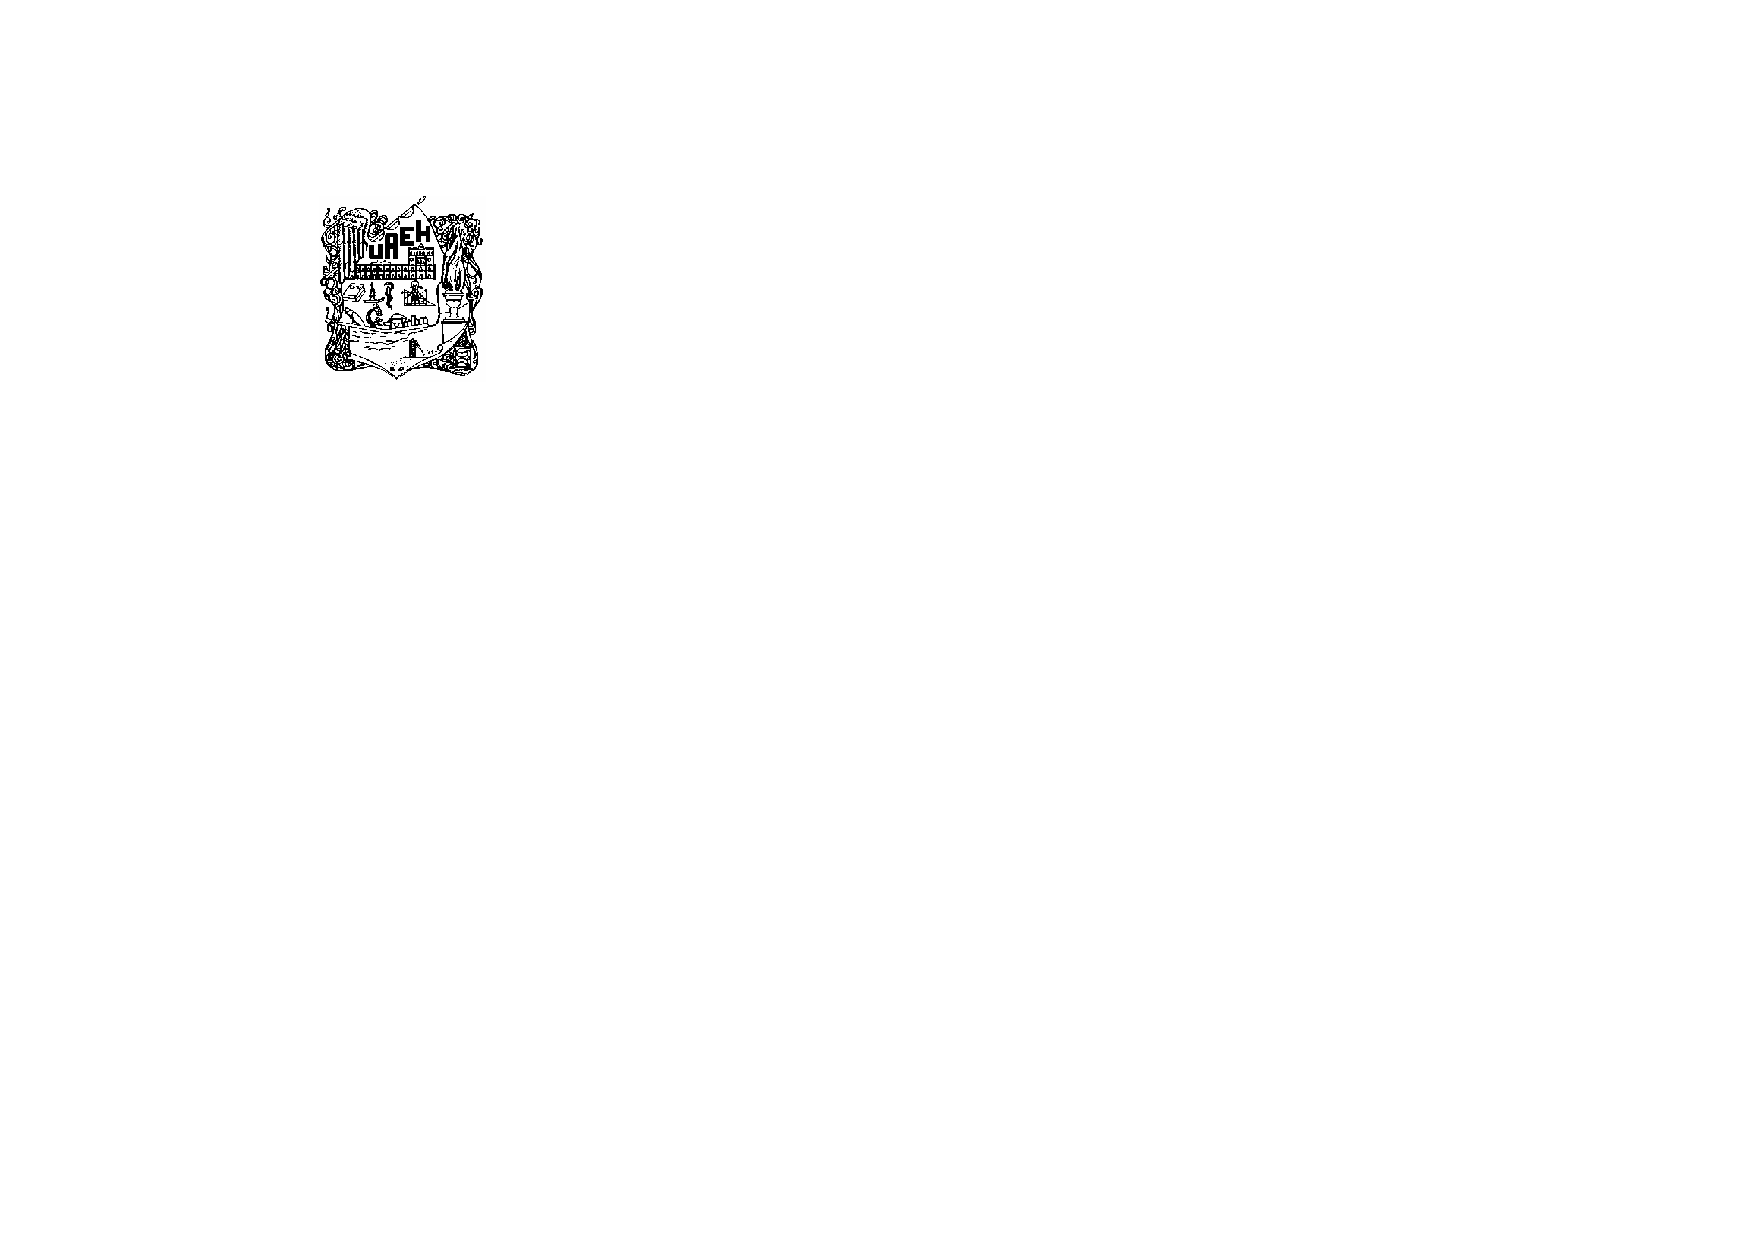
\includegraphics[scale=1.2,bb=55 20 0 0]{escudouaeh.pdf}

    \vspace*{\elespacio}

    \textsc{Universidad Autónoma del Estado de Hidalgo}

    \textsc{Instituto de Ciencias Básicas e Ingeniería}

    \textsc{Área Académica de Matemáticas y Física}

    \vspace*{\elespacio}

    {\Huge\bfseries Un enfoque computacional de representaciones de
      grupos en homologías\par}

    \vspace*{\elespacio}

    {\large Tesis que para obtener el título de}

    \vspace*{\elespacio}

    {\Large\textsc{Licenciado en Matemáticas Aplicadas}}

    \vspace*{\elespacio}

    {\large presenta}

    \vspace*{\elespacio}

    {\Huge Manuel Campero Jurado}

    \vspace*{\elespacio}

    {\large bajo la dirección de}

    \bigskip

    {\Large Dr.~Rafael Villarroel Flores}

    \bigskip

    {Pachuca, Hidalgo. Octubre de 2018.}

    \vspace*{\fill}

  \end{center}
\end{titlepage}

\thispagestyle{empty}
\begin{flushleft}
  {\bfseries\Large Resumen}
\end{flushleft}

En esta tesis se hace blah blah blah blah blah blah blah blah blah
blah blah blah blah blah blah blah blah blah.

\vspace{2cm}

\begin{flushleft}
  {\bfseries\Large Abstract}
\end{flushleft}

In this thesis blah blah blah blah blah blah blah blah blah
blah blah blah blah blah blah blah blah blah.

 \newpage \thispagestyle{empty}

\chapter{Representaciones de grupos}
\label{cha:Representaciones de grupos}

Sea $ \mathrm{GL}(n,\mathbb{C})$ el grupo de todas las matrices no
singulares de grado $n$ sobre el campo de los números complejos
$\mathbb{C}$. Sea $G$ un grupo. Una representación (matricial) de $G$
se define como un homomorfismo:
\begin{equation*}
  A \colon a \mapsto \mathrm{GL}(n,\mathbb{C})
\end{equation*}
el cual por definición cumple
\begin{enumerate}
\item $A\left(ab\right)=A\left(a\right)A\left(b\right)$,
\item $A\left(1\right)=\mathrm{I}$ (la matriz identidad),
\item $A\left(a^{-1}\right)=A\left(a\right)^{-1}$.
\end{enumerate}
El número $n$ se llama el grado de la representación. Se dice que la
representación es fiel, si $A$ es inyectiva.

\textbf{Ejemplo 1.1.} El mapeo que manda cada elemento de $G$ a $1
\in \mathbb{C}$ es una representación de grado 1. Ésta es llamada la
representación unitaria de $G$, y es denotada por $1_{G}$.

\textbf{Ejemplo 1.2.} Dada una representación $A\left(a\right)$, el mapeo
\begin{equation*}
  a \mapsto P^{-1}A\left(a\right)P
\end{equation*}  
se convierte en una representación de $G$ para cualquier matriz $P$ no singular.

Sean $A$ y $B$ representaciones de $G$. Si existe una
matriz no singular $P$ tal que para todo $a \in G$:
\begin{equation*}
  B\left(a\right)= P^{-1}A\left(a\right)P
\end{equation*}
diremos que $A$ y $B$ son equivalentes. Representaciones equivalentes
se denotan como $A \sim B$. La relación $\sim$
define una clase de equivalencia de representaciones de $G$.

\textbf{Ejemplo 1.3.} Sea $S_{n}$ el grupo simétrico de grado
$n$. Para un elemento
\begin{equation*}
  \sigma =
  \begin{pmatrix}
    1 & 2 & \cdots  & n\\ 
    s_{1} & s_{2} & \cdots & s_{n}
  \end{pmatrix} 
  \in S_{n}
\end{equation*}  
Sea $A\left(\sigma\right)$ la matriz cuyo $i$-ésimo renglón es
$\left(0,...,0,1,0,...,0\right)$ con 1 en el $s_{i}$-ésimo lugar,
entonces para $\left(i,j=1,2,...,n\right)$, se tiene:
\begin{equation*}
A\left(\sigma\right) = \left(\alpha_{ij}\left(\sigma\right)\right) 
\end{equation*}
con
\begin{equation*}
         \alpha_{ij}\left(\sigma\right) = \left\{
	       \begin{array}{ll}
		 1      & \mathrm{si\ } j = s_{i} \\
		 0      & \mathrm{otro\ caso\ } 
	       \end{array}
	     \right.
\end{equation*}
El mapeo $\sigma \mapsto A\left(\sigma\right)$ es una representación
fiel de $S_{n}$.

\textbf{Ejemplo 1.4.} Sea $G$ un grupo finito que
consiste de los elementos $a_{1},a_{2},...,a_{n}$ y sea $S^{G}$ el
grupo simétrico en $G$. El mapeo lleva cada elemento de $a \in G$ a la
permutación
\begin{equation*}
  \begin{pmatrix}
    a_{1} & a_{2} & \cdots  & a_{n}\\ 
    a_{1}a & a_{2}a & \cdots & a_{n}a
  \end{pmatrix} 
  \in S_{n}^{G},
\end{equation*}
el cual, es un homomorfismo inyectivo de $G$ a $S^{G}$. A la permutación
anterior, se le asocia la siguiente matriz:
\begin{equation*}
  A(a)=\big(\alpha_{ij}(a)\big)
\end{equation*}
con
\begin{equation*}
         \alpha_{ij}\left(a\right) = \left\{
	       \begin{array}{ll}
		 1      & \mathrm{si\ } a_{i}a = a_{j} \\
		 0      & \mathrm{otro\ caso\ } 
	       \end{array}
	     \right.
\end{equation*}
como en el ejemplo 1.3. Entonces el mapeo
$a \mapsto A\left(\sigma\right)$ convierte una representación fiel de
$G$. Ésta representación es llamada representación regular derecha de
$G$. Sea $\delta\left(a\right)$
\begin{equation*}
         \alpha_{ij}\left(a\right) = \left\{
	       \begin{array}{ll}
		 1      & \mathrm{si\ } a = 1 \\
		 0      & \mathrm{otro\ caso.\ } 
	       \end{array}
	     \right.
\end{equation*}
Entonces
\begin{equation*}
  A\left(a\right) = 
  \begin{pmatrix}
    \delta\left(a_{1}aa_{1}^{-1}\right) & \delta\left(a_{1}aa_{2}^{-1}\right) & \cdots  & \delta\left(a_{1}aa_{n}^{-1}\right)\\
    \delta\left(a_{2}aa_{1}^{-1}\right) & \delta\left(a_{2}aa_{2}^{-1}\right) & \cdots  & \delta\left(a_{2}aa_{n}^{-1}\right)\\ 
    \vdots & \vdots & \ddots & \vdots\\
    \delta\left(a_{n}aa_{1}^{-1}\right) & \delta\left(a_{n}aa_{2}^{-1}\right) & \cdots  & \delta\left(a_{n}aa_{n}^{-1}\right)
  \end{pmatrix} 
\end{equation*}
Si a $\neq$ 1, cada entrada sobre la diagonal es cero.

La representación regular izquierda de $G$ se define análogamente
usando el siguiente homomorfismo:
\begin{equation*}
  a \mapsto
  \begin{pmatrix}
    a_{1} & a_{2} & \cdots  & a_{n}\\ 
    aa_{1} & aa_{2} & \cdots & aa_{n}
  \end{pmatrix}
\end{equation*}
concretamente
\begin{equation*}
  A\left(a\right) = 
  \begin{pmatrix}
    \delta\left(a_{1}^{-1}aa_{1}\right) & \delta\left(a_{1}^{-1}aa_{2}\right) & \cdots  & \delta\left(a_{1}^{-1}aa_{n}\right)\\
    \delta\left(a_{2}^{-1}aa_{1}\right) & \delta\left(a_{2}^{-1}aa_{2}\right) & \cdots  & \delta\left(a_{2}^{-1}aa_{n}\right)\\ 
    \vdots & \vdots & \ddots & \vdots\\
    \delta\left(a_{n}^{-1}aa_{1}\right) & \delta\left(a_{n}^{-1}aa_{2}\right) & \cdots  & \delta\left(a_{n}^{-1}aa_{n}\right)
  \end{pmatrix} 
\end{equation*}
Sea $\phi \colon a \mapsto \phi\left(a\right)$ un homomorfismo de $G$
en $S_{n}$ (es decir, una representación permutación de
$G$). Expresando la permutación $\phi\left(a\right)$ por la matriz
$A\left(a\right)$ como en el ejemplo 1.3, se obtiene una
representación matricial.

Sea $A$ una representación de grado $n$. Se dice que $A$ es reducible
si hay una matriz no singular, tal que
\begin{equation*}
  P^{-1}A\left(a\right)P=
  \begin{pmatrix}
    B\left(a\right) & 0 \\
    D\left(a\right) & C\left(a\right)
  \end{pmatrix}, 
\end{equation*}  
donde $B\left(a\right)$, $C\left(a\right)$ son matrices cuadradas de
grado $r$, $s$ con $r \geq 1$, $s \geq 1$, $r+s=n$. Observe que $B$ y
$C$ son representación de $G$ de grado $r$, $s$
respectivamente. Además se tiene que las representaciones
\begin{equation*}
  A_{1}\left(a\right)=
  \begin{pmatrix}
    B\left(a\right) & 0 \\
    D\left(a\right) & C\left(a\right)
  \end{pmatrix}
\end{equation*}
y
\begin{equation*} 
   A_{2}\left(a\right)=
  \begin{pmatrix}
    C\left(a\right) & D\left(a\right) \\
    0 & C\left(a\right)
  \end{pmatrix}
\end{equation*}
son equivalentes, porque
$Q^{-1}A_{1}\left(a\right)Q=A_{2}\left(a\right)$, con
\begin{equation*}
  Q=
  \begin{pmatrix}
    0 & I_{r} \\ 
    I_{s} & 0
  \end{pmatrix},
\end{equation*}
donde $ \mathrm{I_{r}}$, $ \mathrm{I_{s}}$ son matrices identidad de
grado $r$, $s$ respectivamente.

Si $A$ no es reducible, se dice que $A$ es irreducible . En el ejemplo
1.3, el mapeo $a \mapsto B\left(a\right)$ y
$a \mapsto C\left(a\right)$ se convierten en representaciones de grado
$r$, $s$, respectivamente.

Dada una representación de $G$, $A$, y $B$, con grado $n$, $m$,
respectivamente, el mapeo.
\begin{equation*}
  Q=
  \begin{pmatrix}
    A\left(a\right) & 0 \\ 
    0 & B\left(a\right)
  \end{pmatrix}, \qquad \mathrm{para\ todo\ } a \in G
\end{equation*}
se convierte en una representación de $G$ de grado $n+m$. Esta
representación es llamada la suma directa de $A$ y
$B$, y es denotada por $A \oplus B$.

Una representación $A\left(a\right)$ de $G$ se dice completamente
reducible si $A$ es equivalente a la suma directa de algunas
representaciones irreducibles, es decir, existe una matriz no singular
$P$, tal que

\begin{equation*}
 P^{-1}A\left(a\right)P=
 \begin{pmatrix}
   F_{1} \left(a\right) & & & & & 0\\
   & F_{2} \left(a\right) & & & & \\
   & & . & & & \\
   & & & . & & \\
   & & & & . & \\
   0 & & & & & F_{r} \left(a\right)
 \end{pmatrix}
\end{equation*}
donde cada $F_{i}\left(a\right)$ con $i=1,2,...,r$ es una
representación irreducible de $G$.

\subsubsection{Representación por matrices unitarias, y
  representaciones de completamente reducibles de grupos finitos}
Una representación $A$ de $G$ se dice unitaria si $A\left(a\right)$ es
una matriz unitaria para todo $a \in G$, lo cual significa que
$\overline{A\left(a\right)}^{t}A\left(a\right)=I$. Aquí
$\overline{A\left(a\right)}^{t}$ denota la transpuesta de
$\overline{A}=\left(\alpha_{ij}\right)$, donde
$A=\left(\alpha_{ij}\right)$, y $\overline{\left(\alpha_{ij}\right)}$
es el complejo conjugado de $\left(\alpha_{ij}\right)$. Se pretende
mostrar que cada representación de un grupo finito es equivalente a
una representación unitaria y es completamente reducible.

Una matriz se dice hermitiana si $\overline{A^{t}}=A$, y positiva
definida si $\overline{x}^{t}Ax>0$ para todo vector columna $x$
(distinto de cero).

\textbf{Lema 2.1.} Para cualquier matriz no singular $A$,
$\overline{A\left(a\right)}^{t}A$ es una matriz hermitiana definida
positiva. La suma de matrices hermitianas definidas positivas, también
es hermitiana y definida positiva.

\textbf{Lema 2.2.} Para cualquier matriz hermitiana definida positiva
$A$, existe una matriz triangular superior no singular $C$ tal que
$\overline{C}^{t}AC=\mathrm{I}$.
\begin{proof}
  sea $A\left(\alpha_{ij}\right)$ para
  $\left(i,j=1,2,...,n\right)$. Entonces
  $\alpha_{ji}=\overline{\alpha_{ij}}$ y
  $\left(\alpha_{ii}\right)>0 \quad \mathrm{para\ }$. Entonces $A$
  tiene la forma
\begin{equation*}
  A=
  \begin{pmatrix}
    \alpha & a \\ 
    \overline{a}^{t} & \mathrm{B}
  \end{pmatrix}
\end{equation*}
para $\alpha=\alpha_{11}>0$,
$ a= \left(\alpha_{12},\alpha_{13},...,\alpha_{1n} \right) $,
$ \mathrm{B}=\left(\alpha_{ij}\right)$, $ \left(i,j=2,...,n\right) $.
\begin{equation*} 
  C_{1}=
  \begin{pmatrix}
    \frac{1}{\sqrt{\alpha}} & -\frac{1}{\alpha} \\ 
    0 & \mathrm{I}
  \end{pmatrix}
\end{equation*}
entonces, 
\begin{equation*}
  \overline{C_{1}}^{t}AC_{1} =
  \begin{pmatrix}
    1 & 0 \\ 
    0 & -\frac{1}{\alpha}\overline{a}^{t}a+\mathrm{B}
  \end{pmatrix}
\end{equation*}  
y $-\frac{1}{\alpha}\overline{a}^{t}a+\mathrm{B}$ es una matriz
hermitiana definida positiva. Y la prueba se sigue usando inducción el
grado de $A$ veces.
\end{proof}

\textbf{Teorema 2.3.} Sea $G$ un grupo finito. Para una representación
$F$ de $G$, entonces existe una matriz triangular superior no singular $C$, tal que
$C_{-1}F\left(a\right)C$ es una matriz unitaria para todo $a \in G$.
\begin{proof}
Sea
\begin{equation*}
A=\sum_{b \in G} \overline{F\left(b\right)}^{t}F\left(b\right)
\end{equation*}
Entonces $A$ es una matriz hermitiana definida positiva por el Lema
2.1. Entonces existe una matriz triangular no singular $C$, tal que

\begin{equation*}
  \overline{C}^{t}AC= I
\end{equation*}
\begin{equation*}
  A=(\overline{C}^{t})^{-1}C^{-1}.
\end{equation*}
Ya que
\begin{equation*}
\overline{F\left(a\right)}^{t}AF\left(a\right)=\sum_{b \in G} \overline{F\left(ba\right)}^{t}F\left(ba\right)=A
\end{equation*},
se obtiene
\begin{equation*}
\overline{F\left(a\right)}^{t}(\overline{C}^{t})^{-1}C^{-1}F\left(a\right)=(\overline{C}^{t})^{-1}C^{-1}
\end{equation*},
es decir\\~\\
\begin{equation*}
\overline{(C^{-1}F(a)C)}^{t}(C^{-1}F(a)C)=I
\end{equation*}
y $C^{-1}F(a)C$ es una matriz unitaria.
\end{proof}

\textbf{Teorema 2.4.} Una representación de un grupo finito es
completamente reducible.

Sea $A$ una representación de un grupo finito de $G$ y sea $A(a)$
descompuesta como
\begin{equation*}
  A(a)=
  \begin{pmatrix}
    A_{1}(a) & * \\ 
    0 & A_{2}(a)
  \end{pmatrix}.
\end{equation*}

\begin{proof}
  Por el teorema anterior, existe una matriz triangular no superior
  $C$ tal que $C^{-1}A(a)C$ es una matriz unitaria. Sea
  $U(a)=C^{-1}A(a)C$. Como $C$ es una matriz triangular superior,
  $U(a)$ se descompone como
\begin{equation*}
  U(a)=
  \begin{pmatrix}
    U_{1}(a) & V(a) \\ 
    0 & U_{2}(a)
  \end{pmatrix}
\end{equation*}  
Como $\overline{U(a)}^{t}=U(a)^{-1}=U(a^{-1})$, se obtiene
\begin{equation*}
  \begin{pmatrix}
    \overline{U_{1}(a)}^{t} & 0 \\ 
    \overline{V(a)}^{t} & \overline{U_{2}(a)}^{t}
  \end{pmatrix}
  =
  \begin{pmatrix}
    U_{1}(a^{-1}) & V(a^{-1}) \\ 
    0 & U_{2}(a^{-1})
  \end{pmatrix}
\end{equation*}
\end{proof}

\textbf{Lema 3.1.} (Lema de Schur) Sea $A$ y $B$ representaciones
irreducibles de un grupo $G$ con grados $m$ y $n$ respectivamente. Sea
$P$ una matriz de $m$x$n$ con la propiedad de que $A(a)P=PB(a)$, para
todo $a \in G$.  entonces:
\begin{enumerate}
\item $P=0$
\item $m=n$ y $P$ es no singular.
\end{enumerate}

\begin{proof}
Asumimos $P \neq 0$. Y se quiere mostrar la segunda
condición. Supongamos que $m \neq n$, o $m=n$ y $P$ es
singular. Entonces existe $Q \in \mathrm{GL}(m,\mathbb{C})$ y
$R \in \mathrm{GL}(n,\mathbb{C})$, tal que
\begin{equation*}
  QPR=
  \begin{pmatrix}
    I_{r} & 0 \\ 
    0 & 0
  \end{pmatrix} 
\end{equation*}
donde $I_{r}$ es la matriz identidad de grado $r$. con
$r<$max$\left\{ m,n \right\}$. Como
$QA(a)Q^{-1}(QPR) = QPR(R^{-1}B(a)R)$, y se obtiene
\begin{equation*}
  \begin{pmatrix}
    A_{11} & 0 \\ 
    A_{21} & 0
  \end{pmatrix}
  =
  \begin{pmatrix}
    B_{11} & B_{12} \\ 
    0 & 0
  \end{pmatrix},
\end{equation*}
donde
\begin{equation*}
  QA(a)A^{-1}=
  \begin{pmatrix}
    A_{11} & A_{12} \\ 
    A_{21} & A_{22}
  \end{pmatrix} 
\end{equation*}  
con $A_{11}$ una matriz cuadrada de grado $r$. Y
\begin{equation*}
  R^{-1}B(a)R=
  \begin{pmatrix}
    B_{11} & B_{12} \\ 
    B_{21} & B_{22}
  \end{pmatrix}
\end{equation*}
con $B_{11}$ una matriz cuadrada de grado $r$. Por lo tanto
$A_{21}=0$ si $r<m$ y $B_{12}$ si $r<n$. De cualquier manera
$\mathbb{A}$ o $\mathbb{B}$ es reducible, lo cual es una
contradicción.
\end{proof}

\textbf{Teorema 3.2.} Sea $A$ una representación irreducible de un
grupo $G$. Sea $P$ una matriz con la propiedad $A(a)P=PA(a)$ para todo
$a \in G$. Entonces $P=\lambda I$, para algún
$\lambda \in \mathbb{C}$.
\begin{proof}
  Sea $\lambda$ un valor propio de $P$. Entonces
  det$(\lambda I - P)=0$, y además para todo $a \in G$
  \begin{equation*}
    A(a)(\lambda I - P)=(\lambda I - P)A(a)
  \end{equation*}
  Entonces por el Lema de Schur,
  \begin{equation*}
    \lambda I-P=0
  \end{equation*}
\end{proof}

\textbf{Teorema 3.2.} Sea $G$ un grupo abeliano. Entonces cada
representación irreducible de $G$ es de grado 1.

\begin{proof}
  Sea $A$ una representación irreducible de $G$. Como $A(a)$ conmuta
  con $A(b)$, el teorema pasado nos dice que $A(a)=\lambda(a) I$ para
  algún $\lambda(a) \in \mathbb{C}$. Entonces $A$ es irreducible, y su
  grado debe ser $1$.
\end{proof}

\textbf{(Relación ortogonal de caracteres).} Desde aquí en adelante,
se asumirá que estamos trabajando con grupos finitos.

\textbf{Caracteres} Para una matriz cuadrada $A=\alpha_{ij}$ de grado
$n$, tr$A$ denota la traza de $A$, es decir
\begin{itemize}
  \item tr$A= \alpha_{11}+ \alpha_{22} + \cdots + \alpha_{nn}$.
\end{itemize}
Cálculos directos muestran que

\textbf{Lema 4.1. }
\begin{enumerate}
\item tr$(AB)$=tr$(BA)$.
\item tr$(P^{-1}AP)=tr$(A), para alguna matriz no singular $P$.
\end{enumerate}

Para una representación $A$ de un grupo $G$, sea
tr$A(a)=\chi(a)$. Entonces $\chi(a)$ es una función que toma valores
en $\mathbb{C}$ y es llamada el carácter de $A$. Obviamente, $\chi(1)$
es igual al grado de $A$. Caracteres de representaciones irreducibles
son llamados caracteres irreducibles. Y por el lema 4.1(2), se tiene
lo siguiente:

\textbf{Lema 4.2. } Representaciones equivalentes de un grupo tienen
el mismo carácter.

Como $A(x^{-1}ax)=A(x)^{-1}A(a)A(x)$, se sigue que
\begin{equation*}
  \chi(x^{-1}ax)=\chi(a)
\end{equation*}  
Así $\chi$ toma el mismo valor en una clase de conjugación de $G$. Tal
función es llamada función de clase.

\textbf{La primera relación ortogonal de caracteres.} Sea $G$ un grupo
de orden $g$. Sean $A=(\alpha_{ij}(a))$ y $B=(\beta_{ij}(a))$ representaciones irreducibles de $G$ con grado $m,n$,
respectivamente. Para una matriz arbitraria $U=(\gamma_{ij})$, de
$m$x$n$, se tiene

\begin{equation*}
 V=\sum_{x \in G} A(x)UN(x^{-1}).
\end{equation*}
Entonces
\begin{equation*}
  \begin{aligned}
    A(a)V &=\sum_{x \in G} A(ax)UN(x^{-1})\\
    &=\sum_{y \in G} A(y)UB(y^{-1}a) \qquad (y=ax)\\
    &=\sum_{y \in G} A(y)UB(y^{-1})B(a).
  \end{aligned}
\end{equation*}
Como $y$ varía sobre $G$ conforme $x$ lo hace, se tiene
\begin{equation*}
  A(a)V=VB(a).
\end{equation*}  
Asumimos que $A$ y $B$ no son equivalentes. Entonces $V=0$ por el Lema
de Schur. La entrada $(i,j)$ de $V$ es:

\begin{equation*}
 \sum_{x \in G} \sum_{u,v} \alpha_{iu}(x) \gamma_{uv} \beta_{vj}(x^{-1}) = 0.
\end{equation*}
En particular, para algún par de $u$,$v$ sea $\gamma_{uv}=1$ y para
cualquier otro caso $\gamma_{\rho \sigma}=0$. Lo cual conduce a

\begin{equation*}
  \sum_{x \in G} \alpha_{iu}(x) \beta_{vj}(x^{-1}) = 0.
\end{equation*}
Ahora, asumimos que $\mathbb{A}=\mathbb{B}$. Entonces para algún
$\lambda \in \mathbb{C}$, $V=\lambda\mathrm{I}$, y por el Teorema
3.2. La entrada $(i,j)$ de $V$ es:

\begin{equation*}
\qquad \sum_{x \in G} \sum_{u,v} \alpha_{iu}(x) \gamma_{uv} \beta_{vj}(x^{-1}) = \delta_{ij}\lambda,
\end{equation*}
donde $\delta_{ii}=1$, $\delta_{ij}=0$ ($i \neq j$). Tomando la traza de
\begin{equation*}
\qquad \sum_{x \in G} A(x)UA(x^{-1}) = \lambda \mathrm{I}
\end{equation*}
y se obtiene
\begin{equation*}
  g(\gamma_{11}+\gamma_{22}+ \cdots +\gamma_{nn})
\end{equation*}  
donde $n$ es el grado de $\mathbb{A}$, y $g$ es la cardinalidad de $G$, de lo cual se sigue:
\begin{equation*}
\lambda=\frac{g}{n}(\gamma_{11}+\gamma_{22}+ \cdots + \gamma_{nn}).
\end{equation*}

Ahora, para algún par de $u$,$v$ sea $\gamma_{uv}=1$ y para cualquier otro caso $\gamma_{\rho \sigma}=0$. Entonces
\begin{equation*}
  \sum_{x \in G} \alpha_{iu}(x) \beta_{vj}(x^{-1}) = \delta_{ij} \delta_{uv}\frac{g}{n}.
\end{equation*}
Lo cual nos conduce al siguiente teorema

\textbf{Teorema 4.3. } Sea $G$ un grupo de orden $g$.
\begin{itemize}
\item Sea $\mathbb{A}: a \rightarrow A(a)=(\alpha_{ij}(a))$ una
  representación irreducible de $G$ con grado $n$. Entonces
\end{itemize}
\begin{equation*}
\sum_{x \in G} \alpha_{iu}(x) \alpha_{vj}(x^{-1}) = \delta_{ij} \delta_{uv}\frac{g}{n}.
\end{equation*}
\begin{itemize}
\item Sea $\mathbb{B}:b \rightarrow B(a)=(\beta_{ij}(a))$ una
  representación irreducible, la cual no es equivalente a
  $\mathbb{A}$, entonces
\end{itemize}
\begin{equation*}
\sum_{x \in G} \alpha_{iu}(x) \beta_{vj}(x^{-1}) = 0.
\end{equation*}
Sean $\chi$, $\chi^{'}$ los caracteres de $\mathbb{A}$,
$\mathbb{B}$. Por el teorema anterior, poniendo a $u=i$, $v=j$ y
tomando la suma sobre $i$,$j$, se obtiene lo siguiente:

\textbf{Teorema 4.4. } (La primer relación de ortogonalidad de
caracteres) Sea $G$ un grupo de orden $g$.
\begin{itemize}
\item Sea $\chi$ un carácter irreducible de $G$, entonces 
\end{itemize}
\begin{equation*}
\sum_{x \in G} \chi(x) \chi(x^{-1}) = g.
\end{equation*}
\begin{itemize}
\item Sea $\chi$, $\chi^{'}$ caracteres de representaciones
  irreducibles no equivalentes de $G$, entonces
\end{itemize}
\begin{equation*}
\sum_{x \in G} \chi(x) \chi^{'}(x^{-1}) = 0.
\end{equation*}
Se observa que $\chi(a^{-1})=\overline{\chi(a)}$ para todo $a \in G$,
porque el Teorema 2.3 dice que $\mathbb{A}$ es equivalente a una
representación unitaria $\mathbb{U}\colon a \mapsto U(a)$, y se por lo
tanto
\begin{equation*} \label{4.5}
\chi(a^{-1})=trU(a^{-1})=trU(a)^{-1}=tr \overline{U(a)}^{t} = \overline{\chi(a)}  
\end{equation*} 
Sean $\mathbb{F}_{1}$, $\mathbb{F}_{2}$,... representantes de las
clases de equivalencia de las representaciones irreducibles de un
grupo $G$ y sea $\chi_{1}$, $\chi_{2}$,... los caracteres de
$\mathbb{F}_{1}$, $\mathbb{F}_{2}$,... .  Sea $C_{1}$,
$C_{2}$,...,$C_{k}$ las clases de conjugación de $G$ con
$|C_{\alpha}|=h_{\alpha}$ ($\alpha=1, 2, 3,...,k$) y sea $a_{1}$,
$a_{2}$,...,$a_{k}$ los representantes de las clases de
conjugación. Como los caracteres son funciones de clases, el Teorema
4.4 se reescribe como sigue

\textbf{Teorema 4.4'. }
\begin{equation*}
\sum_{\alpha=1}^{k} h_{\alpha} \chi_{i}(a_{\alpha}) \overline{\chi_{j}(a_{\alpha})} = \delta_{ij}g.
\end{equation*}
Para funciones $\varphi$, $\psi$ que toman valores en $\mathbb{C}$ en
un grupo $G$ de orden $g$, se define el producto interno
$(\varphi,\psi)_{G}$ de la siguiente manera
\begin{equation*}
(\varphi,\psi)_{G} = \frac{1}{g} \sum_{x \in G} \varphi(x) \psi(x^{-1})
\end{equation*}
Cuando sea claro que se está hablando del grupo $G$, se escribirá
$(\varphi,\psi)$ en lugar de $(\varphi,\psi)_{G}$. Claramente el
producto interno cumple las siguientes propiedades
\begin{equation*}
  \begin{aligned}
    (\varphi,\psi) &= (\psi,\varphi), \\
    (\varphi_{1}+\varphi_{2},\psi) &= (\varphi_{1},\psi)+(\varphi_{2},\psi), \\
    (\varphi,\psi_{1}+\psi_{2}) &= (\varphi,\psi_{1})+(\varphi,\psi_{2}), \\
    (\lambda \varphi,\psi) &= (\psi,\lambda \varphi)=\lambda (\varphi,\psi).
    \end{aligned}
\end{equation*}
Con esta notación la primera relación de ortogonalidad de caracteres
es expresada como sigue:

\textbf{Teorema 4.4''. } Sean $\chi_{1}$, $\chi_{2}$,... los
caracteres de caracteres de representaciones no equivalentes de un
grupo $G$. Entonces
\begin{equation*}
(\chi_{i},\chi_{j})=\delta_{ij}
\end{equation*} 
Multiplicidad de representaciones irreducibles. Sea $\mathbb{A}$ una
representación de un grupo $G$. Como $\mathbb{A}$ es completamente
reducible, entonces por el Teorema 2.3, $\mathbb{A}$ es equivalente a
\begin{equation*}
\begin{aligned}
\begin{pmatrix}
\mathbb{F}_{1} & & & & & & 0\\ 
 & \ddots & & & & & \\
 & & \mathbb{F}_{1} & & & & \\
 & & & \mathbb{F}_{2} & & & \\
 & & & & \ddots & & \\
 & & & & & \mathbb{F}_{2} & \\
0 & & & & & & \ddots
\end{pmatrix},
\end{aligned}
\end{equation*}
donde $\mathbb{F}_{1}$, $\mathbb{F}_{2}$,... son representaciones no
equivalentes. El número $m_{i}$ es llamado la multiplicidad de
$\mathbb{F}_{i}$ en $\mathbb{A}$ ($m_{i}=0$ si $\mathbb{F}_{i}$ no
aparece) y se escribe
\begin{equation*}
\mathbb{A} \sim m_{1} \mathbb{F}_{1}+m_{2} \mathbb{F}_{2}+ \cdots
\end{equation*}
Sea $\chi$ el carácter de $\mathbb{A}$ y $\chi_{i}$ el carácter de $\mathbb{F}_{i}$ ($i = 1, 2, ...$). Entonces
\begin{equation*}
\chi =m_{1} \chi_{1}+ m_{2} \chi_{2}+ \cdots
\end{equation*}
Si $m_{i} \neq 0$, $\mathbb{F}_{i}$ y $\chi_{i}$ son llamados
componentes irreducibles de $\mathbb{A}$ y $\chi$ respectivamente.

\textbf{Teorema 4.5. } Sea $G$ un grupo y sea $\chi$ el carácter de una
representación de $G$. Sea $m_{i}$ la multiplicidad de un carácter
irreducible $\chi_{i}$ en $\chi$. Entonces
\begin{equation*}
m_{i} = (\chi,\chi_{i}) = \frac{1}{g} \sum_{x \in G} \chi(x) \overline{\chi_{i}(x)}
\end{equation*}
Sea $$\chi=\sum_{j} m_{j} \chi_{j}$$ la suma de caracteres
irreducibles con $m_{j}$ la multiplicidad de $\chi_{j}$. Entonces
\begin{equation*}
(\chi,\chi_{i}) = \sum_{j} m_{j} (\chi_{j},\chi_{i})
\end{equation*}

\textbf{Teorema 4.6. } Sean $\mathbb{A}$, $\mathbb{B}$
representaciones de un grupo $G$, y sean $\chi$, $\chi^{'}$ los
caracteres de $\mathbb{A}$, $\mathbb{B}$ respectivamente. Entonces
$\mathbb{A}$, $\mathbb{B}$ son equivalentes si y sólo si
$\chi=\chi^{'}$.

\begin{proof}
  Por el teorema pasado, las multiplicidades de $\mathbb{F}_{i}$ en
  $\mathbb{A}$ y $\mathbb{B}$ son determinadas por los caracteres de
  $\mathbb{A}$ y $\mathbb{B}$. Como cualquier representación de $G$ es
  completamente reducible, $\mathbb{A}$ y $\mathbb{B}$ son
  equivalentes si y sólo si cada representación $\mathbb{F}_{i}$ tiene
  la misma multiplicidad en $\mathbb{A}$ y $\mathbb{B}$. Entonces
  $\mathbb{A} \sim \mathbb{B}$ si y sólo si $\chi=\chi^{'}$.
\end{proof}

Sea $\pi$ el carácter de la representación regular derecha de un grupo
$G$ de orden $g$. Se observa que

\begin{equation*} \label{PR}
         \pi(a) = \left\{
	       \begin{array}{ll}
		 g      & \mathrm{si\ } a = 1 \\
		 0      & \mathrm{otro\ caso\ } 
	       \end{array}
	     \right.
\end{equation*}

Para el carácter $\chi_{i}$ de cada representación irreducible
$\mathbb{F}_{i}$, se sigue que
\begin{equation*}
  \begin{aligned}
    (\pi,\chi_{i}) & =\frac{1}{g} \sum_{x \in G} \pi(x) \overline{\chi_{i}(x)} \\
    &=\frac{1}{g} \pi(1) \chi_{i}(1) \\
    &=\chi_{i}(1) 
  \end{aligned}
\end{equation*}
donde $\chi_{i}(1)$ es el grado de $\mathbb{F}_{i}$. Y por lo tanto se
sigue el siguiente Teorema.

\textbf{Teorema 4.7.} Sea $\pi$ el carácter de la representación
regular derecha. Entonces cada representación irreducible
$\mathbb{F}_{i}$ de $G$ tiene multiplicidad $f_{i}$, donde $f_{i}$ es
el grado de $\mathbb{F}_{i}$. Asi que
\begin{equation*}
  \pi=\sum_{i} f_{i} \chi_{i},
\end{equation*}

donde la suma es sobre todos los caracteres irreducible $\chi_{i}$ de $G$.

La representación regular derecha e izquierda son equivalentes, ya que
el carácter $\pi^{'}$ de la representación regular satisface lo mimo
que $\pi$ y por ello, $\pi = \pi^{'}$.

\textbf{Teorema 4.8.} Sean $\chi_{1}, \chi_{2},...,\chi_{l} $ todos
los caracteres irreducibles de un grupo $G$, que además son distintos
entre sí. Sea $f_{i}$ el grado de $\chi_{i}$ ($i=1, 2,..., l$) y sea
$g$ el orden de $G$. Entonces

\begin{equation*}
  g=f_{1}^{2}+f_{2}^{2}+ \cdots + f_{l}^{2},
\end{equation*}
y para $a \neq 1$,
\begin{equation*}
  f_{1} \chi_{1}(a)+f_{2} \chi_{2}(a)+ \cdots + f_{l} \chi_{l}(a) = 0.
\end{equation*}

\begin{proof}
  Simplemente se debe evaluar
  \begin{equation*}
   \pi=\sum_{i} f_{i} \chi_{i},
 \end{equation*}
 recordando \ref{PR}
\end{proof}

\textbf{La segunda relación de ortogonalidad de caracteres.} Sea $G$
un grupo y sean
$\mathbb{C}_{1}=\left\{1 \right\}, \mathbb{C}_{2},...,\mathbb{C}_{k}$
las clases de conjugación de $G$. Para una clase de conjugación
$\mathbb{C}_{\alpha}$, se define la suma de los elementos de
$\mathbb{C}_{\alpha}$ como:

\begin{equation*}
  \mathbb{C}_{\alpha}=a_{1}+a_{2}+ \cdots + a_{h_{\alpha}} \qquad (h_{\alpha}=|\mathbb{C}_{\alpha}|).
\end{equation*}

Y se define el producto de $\mathbb{C}_{\alpha}$ y $\mathbb{C}_{\beta}$ por
\begin{equation*} \label{MULT}
  \mathbb{C}_{\alpha} \mathbb{C}_{\beta} = \sum_{\gamma=1}^{k} t_{\alpha \beta \gamma} \mathbb{C}_{\gamma}
\end{equation*}

Sea $\mathbb{F} \colon a \mapsto F(a)$ una representación irreducible
de $G$ y sea $f$ el grado de $\mathbb{F}$. Se define
$\mathbb{F} (\mathbb{C}_{\alpha})$ por

\begin{equation*}
  \mathbb{F} (\mathbb{C}_{\alpha}) = \sum_{a \in C_{\alpha}} \mathbb{F}(a).
\end{equation*}

Entonces 
\begin{equation*}
  F(x)^{-1}F(\mathbb{C}_{\alpha})F(x)=\sum_{a \in C_{\alpha}}F(x^{-1}ax)=F(\mathbb{C}_{\alpha}),
\end{equation*}

ya que $x^{-1}ax$ varia sobre $C_{\alpha}$ mientras $a$ lo
hace. Entonces la matriz $\mathbb{F} (\mathbb{C}_{\alpha})$ conmuta
con cada $F(x)$, y por el Teorema 3.2, se llega a que,
\begin{equation*}
   \mathbb{F} (\mathbb{C}_{\alpha})=w_{\alpha}\mathrm{I}.
\end{equation*}

Y tomando la traza de la expresión anterior, se tiene
\begin{equation*}
  h_{\alpha}\chi(a_{\alpha})=w_{\alpha}f,
\end{equation*}
\begin{equation*} \label{4.13}
  w_{\alpha}=h_{\alpha}\chi(a_{\alpha})/f,
\end{equation*}

donde $\chi$ es el carácter de $\mathbb{F}$ y
$a_{\alpha} \in C_{\alpha}$, y por \ref{MULT}, se sigue
\begin{equation*}
  \mathbb{F} (\mathbb{C}_{\alpha})  \mathbb{F} (\mathbb{C}_{\beta}) = \sum_{\gamma}^{k} t_{\alpha \beta \gamma} \mathbb{F}(\mathbb{C}_{\gamma}),
\end{equation*}

\begin{equation*}
  w_{\alpha}w_{\beta} = \sum_{\gamma}^{k} t_{\alpha \beta \gamma} w_{\gamma}.
\end{equation*}

Sustituyendo \ref{4.13} en la expresión de arriba se llega a

\begin{equation*}
  \frac{h_{\alpha} \chi(a_{\alpha})}{f} \frac{h_{\beta} \chi(a_{\beta})}{f} = \sum_{\gamma}^{k} t_{\alpha \beta \gamma} \frac{h_{\gamma} \chi(a_{\gamma})}{f},
\end{equation*}

\begin{equation*} \label{4.14}
   \chi(a_{\alpha}) \chi(a_{\beta}) = \sum_{\gamma}^{k} t_{\alpha \beta \gamma} \frac{h_{\gamma}}{h_{\beta} h_{\alpha}} f \chi(a_{\gamma}).
\end{equation*}

Sean $\chi_{1}, \chi_{1},..., \chi_{l}$ caracteres distintos e
irreducibles de $G$, y sea $f_{i}$ el grado de $\chi_{i}$. \ref{4.14}
se es válida para cada $\chi_{i}$. Y tomando la suma sobre $i$, se
llega a que

\begin{equation*}
  \begin{aligned}
    \sum_{i=1}^{l} \chi_{i}(a_{\alpha}) \chi_{i}(a_{\beta}) &= \sum_{\gamma}^{k} t_{\alpha \beta \gamma} \frac{h_{\gamma}}{h_{\beta} h_{\alpha}} (\sum_{i} f_{i} \chi_{i}(a_{\gamma})) \\
    &= t_{\alpha \beta \gamma} \frac{1}{h_{\beta} h_{\alpha}}g \\
    &=  \left\{
	       \begin{array}{ll}
		 g/h_{\alpha}      & \mathrm{si\ } C_{B} = C_{\alpha^{'}} \\
		 0      & \mathrm{otro\ caso\ } 
	       \end{array}
	     \right.
    \end{aligned}
\end{equation*}

Y se llega a

\begin{equation*}
   \sum_{i=1}^{l} \chi_{i}(a_{\alpha}) \chi_{i}(a_{\beta})=\delta_{\alpha \beta} \frac{g}{h_{\alpha}}.
\end{equation*}

El número $g/h_{\alpha}$ es el orden de $\mathrm{N}(a)$, que es el
centralizador de $a_{\alpha}$ en $G$. Ya que
$\chi_{i}(a_{\beta^{'}})=\overline{\chi_{i} (a_{\beta})}$ por
\ref{4.5}, se obtiene lo siguiente:

\textbf{Teorema 4.9. } (La segunda relación de orgonalidad de
caracteres) Sean $\left\{\chi_{i} \right\}$ el conjunto de los
distintos caracteres irreducibles de $G$ y sea
$\left\{a_{\alpha} \right\}$ el conjunto de los representantes de las
clases de conjugación de $G$. Entonces

\begin{equation*}
  \sum_{i} \chi_{i}(a_{\alpha}) \overline{\chi_{i} (a_{\beta})} = \delta_{\alpha \beta} n_{\alpha}
\end{equation*}

donde $n_{\alpha}$ es el orden de $\mathrm{N}(a)$ y lla suma es sobre
todos los caracteres irreducibles $\chi_{i}$ de $G$.

\textbf{Teorema  4.10. } El número de caracteres distintos e irreducibles de $G$ es
igual que el de las clases de conjugación de $G$.

\begin{proof}
  Se tiene que si $A_{mxn}$ y $B_{nxm}$ son matrices , entonces si el
  determinante de la matri $AB_{mxm}$ es distinto de cero, se sigue que $m \leq n$.
  Sean $\chi_{1}, \chi_{2},...,\chi_{l}$ los distintos caracteres irreducibles de $G$ y sean $a_{1},...,a_{k}$ los representantes de las clases de conjugación de $G$. Entonces por el Teorema 4.4.
\begin{equation*}
  \begin{pmatrix}
    \chi_{1}(a_{1}) & \cdots & \chi_{1}(a_{k}) \\ 
    \vdots &  & \vdots \\
    \chi_{l}(a_{1}) & \cdots & \chi_{l}(a_{k})
  \end{pmatrix}
  \begin{pmatrix}
    h_{1} \overline{\chi_{1}(a_{1})} & \cdots & h_{1} \overline{\chi_{l}(a_{1})} \\ 
    \vdots &  & \vdots \\
    h_{k} \overline{\chi_{1}(a_{k})} & \cdots & h_{k} \overline{\chi_{l}(a_{k})}  
  \end{pmatrix}
\end{equation*}
\begin{equation*}
  =
  \begin{pmatrix}
   g & & 0\\ 
     & \ddots & \\
     0 &  & g
  \end{pmatrix}   
  \end{equation*}.
  Así que $l \leq k$. Por el Teorema 4.9,
\begin{equation*}
  \begin{pmatrix}
    \chi_{1}(a_{1}) & \cdots & \chi_{l}(a_{1}) \\ 
    \vdots &  & \vdots \\
    \chi_{l}(a_{k}) & \cdots & \chi_{l}(a_{k})
  \end{pmatrix}
  \begin{pmatrix}
     \overline{\chi_{1}(a_{1})} & \cdots &  \overline{\chi_{l}(a_{1})} \\ 
    \vdots &  & \vdots \\
     \overline{\chi_{1}(a_{k})} & \cdots &  \overline{\chi_{l}(a_{k})}  
  \end{pmatrix},
\end{equation*}

\begin{equation*}
  =
  \begin{pmatrix}
   n_{1} & & 0\\ 
     & \ddots & \\
     0 &  & n_{k}
  \end{pmatrix}
\end{equation*}.
Por ello, $k \leq l$. Así que $k=l$.
\end{proof}

\textbf{Representaciones inducidas} 

Sea $G$ un grupo de orden $g$ y $H$ un subgrupo de $G$ de orden
$h$. Para una función $\psi$ en $G$, $\psi_{H}$ denota la restricción
de $\psi$ a $H$. Si $\psi$ es una función de clase en $G$, entonces
$\psi_{H}$ también es una función de clase en $H$. Si $\psi$ es el
carácter de una representación de $G$ $\mathbb{A}$, se sigue que
$\psi_{H}$ es el caráter de $\mathbb{A}_{H}$, la restricción de
$\mathbb{A}$ a $H$.

Para una función $\theta$ en $H$, se define la función $\theta^{G}$ de
la siguiente manera

\begin{equation*}
  \theta^{G}=\frac{1}{h} \sum_ u{x \in G} \theta(x^{-1}ax)
\end{equation*}
donde $\theta(x^{-1}ax)=0$ si $x^{-1}ax$ no está en H. $\theta^{G}$ es
una función de clase en $G$, aun si $\theta$ no es una función de
clase en $H$. Si $a$ no es el conjungado de ningún elemento de $H$,
entonces $\theta^{G}(a)=0$.

\textbf{Lema 5.1. } Sea $\psi$ una función de clase de $G$, y sea
$\theta$ una función de clase en un subgrupo $H$ de $G$. Entonces

\begin{equation*}
  (\theta^{G},\psi)_{G}= (\theta,\psi_{H})_{H} .
\end{equation*}

\begin{proof}
  \begin{equation*}
    \begin{aligned}
      (\theta^{G},\psi)_{G} &= \frac{1}{g} \sum_{a \in G} \theta^{G}(a) \psi(a^{-1})\\
      &= \frac{1}{gh} \sum_{a \in G} \sum_{x \in G} \theta(x^{-1}ax) \psi(a^{-1})
    \end{aligned}
  \end{equation*}  
  Solamente los elementos $x^{-1}ax \in H$ aportan algo a la suma. Por
  lo cual tomando $a=x \tilde{a} x^{-1}$ con $\tilde{a} \in H$, se
  obtiene
  \begin{equation*}
    \begin{aligned}
      (\theta^{G},\psi)_{G} &= \frac{1}{gh} \sum_{\tilde{a} \in H} \sum_{x \in G} \theta(\tilde{a}) \psi(x \tilde{a}^{-1} x^{-1})\\
      &= \frac{1}{h} \sum_{\tilde{a} \in H} \theta^{G}(a) (\sum_{x \in G} \psi(x \tilde{a}^{-1}x^{-1})) \\
      &= \frac{1}{h} \sum_{\tilde{a} \in H} \theta^{G}(a) \psi(\tilde{a}^{-1}) \\
      &=  (\theta,\psi_{H})_{H}
    \end{aligned}
  \end{equation*}
\end{proof}

Si $\theta$ es el carácter de una representación de $H$, se dirá que
$\theta^{G}$ es el carácter inducido de $G$ y que $\theta^{G}$ es
inducido por $\theta$. Procederemos a demostrar que el carácter
inducido es el carácter de alguna representación de $G$.

Sea $\left\{ a_{1}, a_{2},\ldots,a_{r}\right\}$ el conjunto de los
representantes de las clases laterales izquierdas de $H$ en $G$:

\begin{equation*}
  G = Ha_{1} \cup Ha_{2} \cup \cdots \cup Ha_{r}.
\end{equation*}

Para una representación de $H$
$\mathbb{A} \colon \tilde{a} \mapsto A(\tilde{a})$ con
$\tilde{a} \in H$, se define la matriz $A^{G}(a)$ de la siguiente
manera
\begin{equation*}
  \begin{pmatrix}
    A(a_{1} a a_{1}^{-1}) & A(a_{1} a a_{2}^{-1}) & \cdots &  A(a_{1} a a_{r}^{-1}) \\
    A(a_{2} a a_{1}^{-1}) & A(a_{2} a a_{2}^{-1}) & \cdots &  A(a_{2} a a_{r}^{-1}) \\
    \vdots &  & \vdots \\
    A(a_{r} a a_{1}^{-1}) & A(a_{r} a a_{2}^{-1}) & \cdots &  A(a_{r} a a_{r}^{-1}) \\
  \end{pmatrix},
\end{equation*}

donde $A(x)=0$ si $x$ no está en H. Lo anterior es una generalización
de la representación regular derecha de $G$. Se desea mostrar que para
toda $a \in G$

\begin{equation*}
  \mathbb{A}^{G} \colon a \mapsto A^{G}(a)
\end{equation*}

es una representaicón de $G$ y tiene grado $nr$, donde
$r= \mid G : H \mid$ y $n$ es el grado de $\mathbb{A}$. Para ello sea
$a_{k}^{-1}$ y $x \in G$, entonces
$\left\{ a_{i} x a_{k}^{-1} \mid i = 1, 2, \ldots, r \right\}$ es el
conjunto de representantes de las clases laterales izquierdas de $H$,
y para $i = 1, 2, \ldots, r$ sólo hay una matríz
$A(a_{i} a a_{k}^{-1})$ que es distinta de cero. Análogamente el
conjunto
$\left\{ a_{i} x a_{k}^{-1} \mid k = 1, 2, \ldots, r \right\}$ está
formado por los representantes de las clases laterales derechas de
$H$, y para $ k = 1, 2, \ldots, r$ únicamente una matriz
$A(a_{i} a a_{k}^{-1})$ no es cero. Sea $C_{ik}$ el bloque $(i,k)$ de
la matriz $A^{G}(a)A^{G}(b)$. Por lo tanto

\begin{equation*}
  C_{ik} = \sum_{j=1}^{r} A(a_{i} a a_{j}^{-1}) A(a_{j} b a_{k}^{-1}).
\end{equation*}

Nuestro objetivo es demostrar que $C_{ik}= A(a_{i} ab
a_{k}^{-1})$. Solamente hay un $s \in \left\{1, 2, \ldots, r \right\}$
tal que $a_{i} a a_{s}^{-1} \in H$, e igual, sólo hay un
$t \in \left\{1, 2, \ldots, r \right\}$ tal que
$a_{t} b a_{k}^{-1} \in H$. Si $s=t$, entonces
$C_{ik}=A(a_{i} a a_{t}^{-1}) A(a_{t} b a_{k}^{-1})=A(a_{i} ab
a_{k}^{-1})$. Si $s \neq t$, entonces $C_{ik}=0$ y
$A(a_{i} ab a_{k}^{-1}) = 0$, ya que
$a_{i} ab a_{k}^{-1} = a_{i} ab a_{t}^{-1} \cdot a_{t} b a_{k}^{-1}
\notin H$ . Por lo cual, de cualquier forma
$C_{ik} = A(a_{i} ab a_{k}^{-1})$, y ello implica que
$A^{G}(a)A^{G}(b)=A^{G}(ab)$. Y ya que
$A^{G}(a)A^{G}(a^{-1})=A^{G}(1)=\mathrm{I}$, se sigue que $A^{G}(a)$
es invertible. Entonces es una representación de G.

Sea $\theta$ el carácter de $\mathbb{A}$ y sea $\chi$ el carácter de
$\mathbb{A}^{G}$. Entonces
\begin{equation*}
  \begin{aligned}
    \chi(a) &= \sum_{i=1}^{r} \theta(a_{i} a a_{i}^{-1}) = \sum_{i=1}^{r} \frac{1}{h} \sum_{\tilde{b} \in H} \theta(\tilde{b} a_{i} a a_{i}^{-1} \tilde{b}^{-1})\\
    &= \frac{1}{h} \sum_{x \in G} \theta(x a x^{-1}) \qquad (x=\tilde{b}a_{i})\\
    &= \theta^{G}(a)
  \end{aligned}
\end{equation*}

Entonces se obtiene que $\chi=\theta^{G}$. Se dirá que
$\mathbb{A}^{G}$ es una representación inducida de $G$, y diremos que
$\mathbb{A}^{G}$ es inducida por $\mathbb{A}$. Ésto, nos lleva a lo
siguiente:

\textbf{Teorema 5.2. } Sea $G$ un grupo y $H$ un subgrupo de $G$. Sea
$\mathbb{A}$ una representación de $H$ con grado $n$ y sea $\theta$ el
carácter de $\mathbb{A}$. Entonces la representación inducida
$\mathbb{A}^{G}$ tiene grado $nr$ con $r=\mid G:H \mid$ y el carácter
de $\mathbb{A}^{G}$ es

\begin{equation*}
  \theta^{G}(a)= \sum_{x \in G} \theta(x^{-1} a x)
\end{equation*}
donde $h= \mid H \mid$.

\textbf{Teorema 5.3. (Reciprocidad de Frobenius) } Sea $H$ un subgrupo
de $G$. Y sean $x_{1}, x_{2},\ldots,x_{r}$ lo caracteres irreducibles
de $G$, y sean $\theta_{1},\theta_{2},\ldots,\theta_{s}$ los
caracteres irreducibles de $H$. Entonces

\begin{equation*}
  (\chi_{i})_{H} = \sum_{j} r_{ij} \theta_{j} 
\end{equation*}
si y sólo si 
\begin{equation*}
  \theta_{j}^{G} = \sum_{i} r_{ij} \chi_{j}.
\end{equation*}

Es decir, dadas representaciones irreducibles $\mathbb{A}$ y
$\mathbb{B}$ de $G$ y $H$ respectivamente, $\mathbb{B}$ es una
componente irreducible de $\mathbb{A}_{H}$ con multiplicidad $r$ si y
sólo si $\mathbb{A}$ es un componente irreducible de $\mathbb{B}^{G}$
con multiplicidad $r$.

\begin{proof}
  Sea $(\chi_{i})_{H} = \sum_{l} r_{il} \theta_{l}$ y sea
  $\theta_{j}^{G} = \sum_{k} s_{kj} \chi_{k}$. Por el lema 5.1, se
  sigue que

  \begin{equation*}
    \begin{aligned}
      r_{ij} &= ((\chi_{i})_{H},\theta_{j})_{H} \\
      &= (\chi_{i},\theta_{j}^{G})_{G}\\
      &= s_{IJ}
    \end{aligned}
  \end{equation*}
\end{proof}


\textbf{Producto de representaciones}

Sean $A$ y $B$ matrices cuadradas de grado $n$, $m$ respectivamente y
sea $A=(\alpha_{ik})$. Se define el producto de Kronecker
$A \otimes B$ de $A$ y $B$ por

\begin{equation*}
  \begin{pmatrix}
    \alpha_{11}B & \cdots & \alpha_{1n}B \\ 
    \vdots &  & \vdots \\
    \alpha_{n1}B & \cdots & \alpha_{nn}B
  \end{pmatrix}
\end{equation*}

$A \otimes B$ es una matriz cuadrada de grado $mn$. Y sin gran
dificultad se puede probar

\textbf{Lema 6.1. }
\begin{enumerate}
\item  tr$(A \otimes B)$ = (tr$(A)$)(tr$(B)$)
\item Sean $A$, $A^{'}$ con grado $n$, y sean $B$, $B^{'}$ de grado
  $m$. Entonces $(A \otimes B)(A^{'} \otimes B^{'})$ =
  $(AA^{'})(BB^{'})$.
\end{enumerate}

Sea $\mathbb{A}_{1} \colon a \mapsto A_{1}(a)$ y
$\mathbb{A}_{2} \colon a \mapsto A_{2}(a)$ representaciones de un
grupo $G$. Por el lema 6.1(2), el mapeo

\begin{equation*}
  a \mapsto A_{1}(a) \otimes A_{2}(a)
\end{equation*}

se transforma en una representación de $G$. A esta representación se le llama el producto de $\mathbb{A}_{1}$ y $\mathbb{A}_{2}$, y es denotado por $\mathbb{A}_{1} \otimes \mathbb{A}_{2}$. Sean $\chi_{1}, \chi_2, \chi$ los caracteres de $\mathbb{A}_{1}$, $\mathbb{A}_{2}$, $\mathbb{A}_{1} \otimes \mathbb{A}_{2}$ respectivamente. Por el lema 6.1(1),

\begin{equation*}
  \chi(a)=\chi_{1}(a) \chi_{2}(a)
\end{equation*}
\begin{equation*}
  \chi = \chi_{1} \chi_{2}
\end{equation*}

Sea $\mathbb{F}_{1}, \mathbb{F}_{2}, \ldots, \mathbb{F}_{r}$ las representaciones irreducibles de $G$ y sea $\chi_{i}$ por el carácter de $\mathbb{F}_{i}$. EL mapeo $a \mapsto \overline{F_{i}(a)}$ también es una representación irreducible y su carácter es $\overline{\chi_{i}}$, donde $\overline{\chi_{i}}(a) = \overline{\chi_{i}(a)}$. Y lo denotaremos $\overline{\chi_{i}}=\chi_{i'}$

\textbf{Teorema 6.2. }


\backmatter


\bibliographystyle{plain}
\bibliography{labiblio}

\printindex


\end{document}
